%%%%%%%%%%%%%%%%%%%%%%%%%%%%%%%%%%%%%%%%%%%%%%%%
% E.Pinault-Bigeard - e.pinault-bigeard@upsti.fr
% http://s2i.pinault-bigeard.com
% CC BY-NC-SA 2.0 FR - http://creativecommons.org/licenses/by-nc-sa/2.0/fr/
%%%%%%%%%%%%%%%%%%%%%%%%%%%%%%%%%%%%%%%%%%%%%%%%
\documentclass[11pt]{article}
%%%%%%%%%%%%%%%%%%%%%%%%%%%%%%%%%%%%%%%%%%%%%%%%
% Package UPSTI_Document
%%%%%%%%%%%%%%%%%%%%%%%%%%%%%%%%%%%%%%%%%%%%%%%%

\usepackage{import}
%
%%%%%%%%%%%%%%%%%%%%%%%%%%%%%%%%%%%%%%%%%%%%%%%%
% Package UPSTI_Document
%%%%%%%%%%%%%%%%%%%%%%%%%%%%%%%%%%%%%%%%%%%%%%%%
\usepackage{subcaption}
\usepackage[usenames, svgnames, dvipsnames]{xcolor}
\usepackage{UPSTI_Document}
\usepackage{pgfplots}
\usepackage{import}
\definecolor{darkspringgreen}{rgb}{0.09, 0.45, 0.27}

\newcommandx*{\dessinRepereFigGeo}[5][1=\vx{},2=\vy{},3=\vz{},4=,5=0]
	{
		\draw [->,very thick] (0,0) -- (1,0) ;
		\draw [->,very thick] (0,0) -- (0,1) ;
    \fill[white] (0,0) circle (0.13);
    \draw [->,very thick] (0,0) circle (0.13);
    \ifnumequal{#5}{0} {% z vers nous
      \fill[black] (0,0) circle (0.03);
      \draw [->,thick] (0,0) circle (0.04);
    }{% z vers la feuille
  		\begin{scope} [rotate=45]
  			\draw [-,thick] (0,-0.12) -- (0,0.12) ;
  			\draw [-,thick] (-0.12,0) -- (0.12,0) ;
  		\end{scope}
    }
		\draw [anchor=north west] (1.1,0) node {${#1}$};
		\draw [anchor=south west] (0,1.1) node {${#2}$};
		\draw [anchor=north east] (-0.1,0) node {${#3}$};
		\draw [anchor=north west] (-0.1,-0.1) node {${#4}$};
	}

	\usepackage{array}
	\newcolumntype{L}[1]{>{\raggedright\let\newline\\\arraybackslash\hspace{0pt}}m{#1}}
	\newcolumntype{C}[1]{>{\centering\let\newline\\\arraybackslash\hspace{0pt}}m{#1}}
	\newcolumntype{R}[1]{>{\raggedleft\let\newline\\\arraybackslash\hspace{0pt}}m{#1}}

	\usepackage{pifont}% http://ctan.org/pkg/pifont
\newcommand{\cmark}{\color{green}\ding{51}}%
\newcommand{\xmark}{\color{red}\ding{55}}%
\newcommand{\fmark}{\ding{229}}%
\newcommand{\itemc}{\item[\cmark]}%
\newcommand{\itemx}{\item[\xmark]}%
\newcommand{\itemf}{\item[\fmark]}%

\usepackage{tikz-timing}
\usepackage{circuitikz}
%---------------------------------%
% Paramètres du package
%---------------------------------%

% Version du document (pour la compilation)
% 1: Document prof
% 2: Document élève
% 3: Document à publier
\newcommand{\UPSTIidVersionDocument}{2}

% Classe
% 1: PTSI				6: PSI*			11: TSI2		16: Spé
% 2: PT	(par défaut)	7: MPSI			12: ATS
% 3: PT*				8: MP			13: PC
% 4: PCSI				9: MP*			14: PC*
% 5: PSI				10: TSI1		15: Sup
%\newcommand{\UPSTIidClasse}{2}



% Matière
% 1: S2I (par défaut)    2: IPT     3: TIPE
% 6: Vie au lycée
\newcommand{\UPSTIvariante}{5}
\newcommand{\UPSTIidMatiere}{0}
\newcommand{\UPSTIintituleMatiere}{Automatique}
\newcommand{\UPSTIsigleMatiere}{Autom}
% Type de document
% 0: Custom*				7: Fiche Métho de			14: Document Réponses
% 1: Cours (par défaut)		8: Fiche Synthèse    		15: Programme de colle
% 2: TD     				9: Formulaire
% 3: TP						10: Memo
% 4: Colle					11: Dossier Technique
% 5: DS						12: Dossier Ressource
% 6: DM						13: Concours Blanc
% * Si on met la valeur 0, il faut décommenter la ligne suivante:
%\newcommand{\UPSTItypeDocument}{Custom}
\newcommand{\UPSTIidTypeDocument}{1}

% Titre dans l'en-tête


% Titre dans l'en-tête

\newcommand{\UPSTIvariante}{5}

\newcommand{\UPSTItitreEnTete}{Automatisme industriel}
%\newcommand{\UPSTItitreEnTetePages}{}
\newcommand{\UPSTIsousTitreEnTete}{Introduction aux API}


% Titre
%\newcommand{\UPSTItitrePreambule}{Automatisme industriel}
\newcommand{\UPSTItitre}{La programmation d'un Automate Industriel}

% Durée de l'activité (pour DS, DM et TP)
\newcommand{\UPSTIduree}{3h30}

% Note de bas de première page
%\newcommand{\UPSTInoteBasDePremierePage}{Geoffrey Vaquette}
% Numéro (ajoute " n°1" après DS ou DM)
\newcommand{\UPSTInumero}{2}

% Numéro chapitre
%\newcommand{\UPSTInumeroChapitre}{1}

% En-tête customisé
%\newcommand{\UPSTIenTetePrincipalCustom}{UPSTIenTetePrincipalCustom}

% Message sous le titre
%\newcommand{\UPSTImessage}{Message sous le titre}


% Référence au programme
%\newcommand{\UPSTIprogramme}{\EPBComp \EPBCompP{B1-02}, \EPBCompP{B2-49}, \EPBCompS{B2-50}, \EPBCompS{B2-51}, \EPBCompP{C1-07}, \EPBCompP{C1-08}}

% Si l'auteur n'est pas l'auteur par défaut
%\renewcommand{\UPSTIauteur}{WWOOOOOOWW}

% Si le document est réalisé au nom de l'équipe
%\newcommand{\UPSTIdocumentCollegial}{1}

% Source
\newcommand{\UPSTIsource}{G. Vaquette, H. Discours}

% Version du document
\newcommand{\UPSTInumeroVersion}{0.3}

%-----------------------------------------------
\UPSTIcompileVars		% "Compile" les variables
%%%%%%%%%%%%%%%%%%%%%%%%%%%%%%%%%%%%%%%%%%%%%%%%


% Titre
%\newcommand{\UPSTItitrePreambule}{Automatisme industriel}
\newcommand{\UPSTItitre}{Cablâge des sorties d'un API simple} 
\usetikzlibrary{arrows,automata,circuits.plc.ladder}

\newlength{\ladderskip}
\setlength{\ladderskip}{5\tikzcircuitssizeunit} % 5\tikzcircuitssizeunit = 35pt
\newlength{\ladderrungsep}
\setlength{\ladderrungsep}{.2\ladderskip}
\def\ladderrungend#1{\pgftransformyshift{-#1\ladderskip-\ladderrungsep}}

\ctikzset{
	logic ports=ieee,
	logic ports/scale=0.7,
}



\newcommand{\automaintienMachineEtat}[0]{
\begin{tikzpicture}[->,>=stealth',shorten >=1pt,auto,node distance=3cm,
                    semithick]
  %\tikzstyle{every state}=[fill=none,draw=none,text=white]

  \node[initial,state] (A)              {M1};
  \node[state]         (B) [right of=A] {M2};

  \path (A) edge [bend left]  node {$B_pM$} (B)
        (B) edge [bend left]  node {$B_pA$} (A);
\end{tikzpicture}
}


%%%%%%%%%%%%%%%%%%%%%%%%%%%%%%%%%%%%%%%%%%%%%%%%
% Début du document
%%%%%%%%%%%%%%%%%%%%%%%%%%%%%%%%%%%%%%%%%%%%%%%%
\begin{document}
\UPSTIbuildPage

%\UPSTIobjectif{Durant cette activité, nous allons analyser une trame pour l'envoi d'informations sur une étiquette.}

\tableofcontents
\pagebreak


\section{Introduction}
Afin d'agir sur l'environnement dans lequel il se trouve, un automate doit être capable de mettre en marche des \textbf{actionneurs}. Ces actionneurs sont classiquement associés à des \textbf{pré-actionneurs} qui adaptent et module l'énergie en entrée de l'actionneur. Ce sont ces pré-actionneurs qui reçoivent des ordres en provenance de l'automate.

\UPSTIboiteCentrale{Structure d'une sortie - Exemple : Moteur triphasé}{
	\begin{center}
		\UPSTIprofEleve{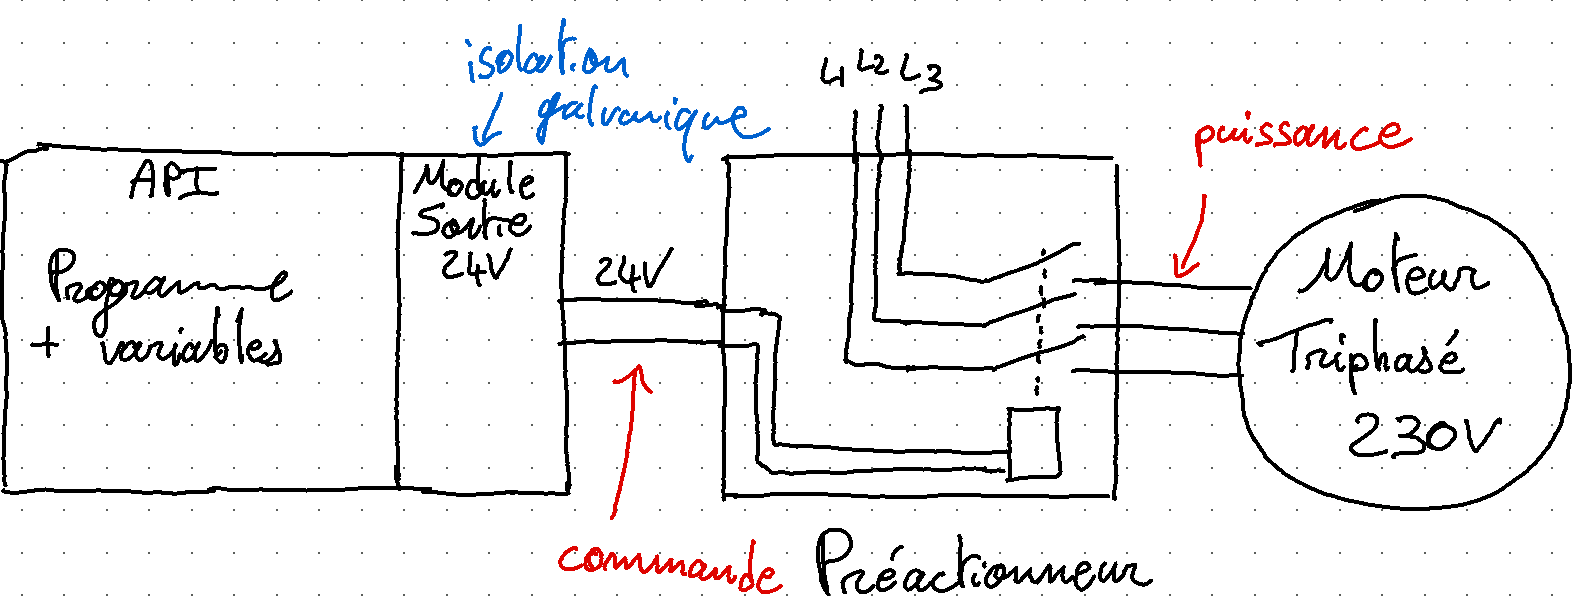
\includegraphics[height=6cm]{images/C05-preActionneur.png}}{\vspace{6cm}}
	\end{center}
}

Comme pour les entrées, il existe différentes technologies d'actionneurs, et avec elles différentes technologies de préactionneurs et donc de modules de sorties.

\section{Sorties logiques}

% \begin{figure}[h!t]
% 	\centering
% 	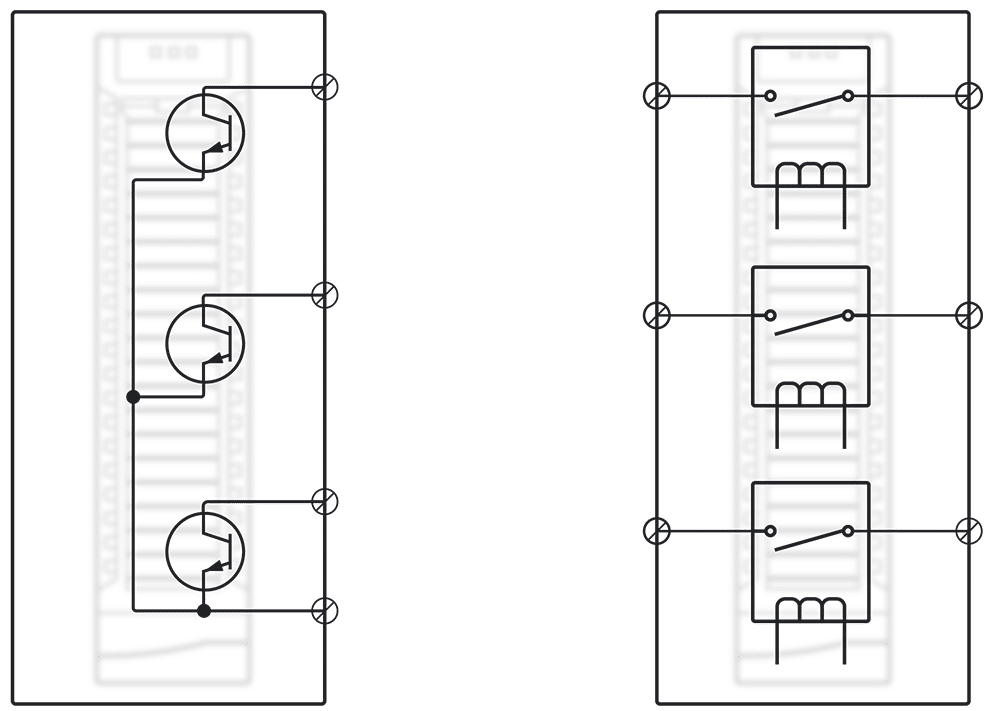
\includegraphics[width=.8\textwidth, height=.2\textheight, keepaspectratio]{images/PLC-Digital-Output-Module-Types.png}
% 	\caption{Sorties à transistor vs Sorties à relais}
% 	\label{fig:typesSortie}
% \end{figure}


\subsection{Les sorties Tout ou Rien}
Pour faire fonctionner des actionneurs Tout ou Rien, il existe deux technologies principales de modules de sorties : Les modules à relais et les modules à transistor.
\subsubsection{Les sorties à relais}

Un module de sorties à relais (ou plus généralement à contacts secs) est composé d'une ou plusieurs sorties chacune commandée par un relais. Pour rappel, un relais peut être vu comme un interrupteur mécanique commandé electriquement.
Le relais assure à la fois l'isolation galvanique (empèche le passage du courant entre le circuit externe et interne du module) et le changement d'état de la sortie. Une sortie à relais comporte deux bornes entre lesquelles se trouve le contact du relais.

D'un point de vue purement fonctionnel il s'agit donc d'un interrupteur mécanique dont l'état (fermé ou ouvert) sera commandé par l'automate en fonction de la valeur de la variable associée à cette sortie.
Dans ce type de module, l'alimentation du préactionneur est alors assurée par une alimentation externe et l'automate a pour unique rôle la commutation du contact.



\begin{figure}[h]
	\centering
	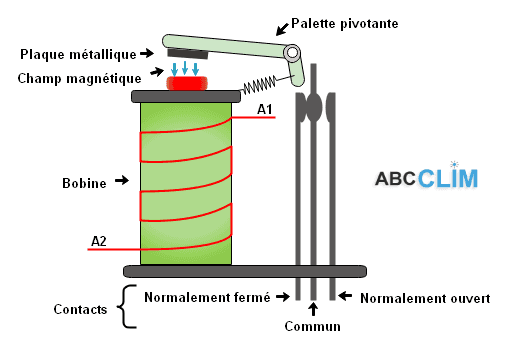
\includegraphics[width=.8\textwidth, height=.15\textheight, keepaspectratio]{images/relais-electromecanique.png}
	\caption{Relais electro-mécanique}
	\label{fig:captPassif}
\end{figure}


\subsubsection{Les sorties électroniques}
Un module de sortie électronique utilise principalement des transistors comme interrupteurs commandés. Ces sorties présentent l'avantage d'être plus rapide en commutation que les sorties à relais.

Contrairement aux sorties à relais, les sorties à transistor ont un point commun (masse ou +Vcc) à toutes les sorties. Chaque sortie ne comporte alors qu'une seule borne sur laquelle on connecte le pré-actionneur désiré.

\begin{figure}[h]
	\centering
	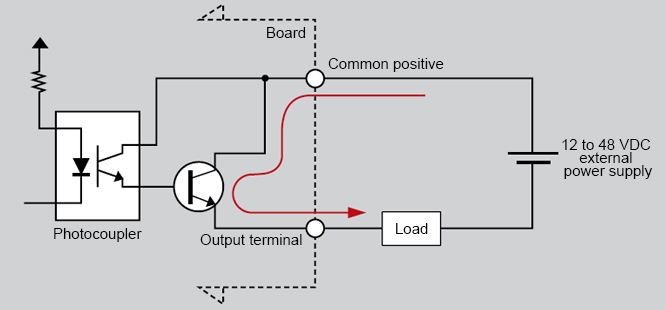
\includegraphics[width=.9\textwidth, height=.25\textheight, keepaspectratio]{images/sortieTransistor.jpg}
	\caption{Sortie à transistor}
	\label{fig:captPassif}
\end{figure}

\UPSTIaRetenir{
	Les principales différences entre les sorties à relais et les sorties à transistor sont :

	\begin{UPSTIaCompleterEnv}
		\begin{tabular}{c|c}
			Sortie à relais                         & Sortie à transistors                     \\\hline
			Libre de potentiel                      & Potentiel imposé par le module de sortie \\
			Fortes puissances                       & Puissances plus faibles                  \\
			Relativement lent (Limité en fréquence) & Plus rapide qu'une sortie à relais       \\
			Nombre de cycle plus Limité				& \\
		\end{tabular}
	\end{UPSTIaCompleterEnv}

	\vspace{2cm}

}

\begin{UPSTIactivite}[][Application]
	\UPSTIquestion{Dessiner le cablâge d'un voyant alimenté par une sortie à relais, puis par une sortie à transistor}
	\vspace{7cm}
\end{UPSTIactivite}

\subsubsection{Les sorties PWM (Pulse Width Modulation)}
Il est possible d'utliser certaines sorties électroniques en modulation de largeur d'impulsion (MLI, ou PWM en anglais). Ce sont des sorties à transistor spécialisées dans la génération de signaux carré dont le programme fera varier le rapport cyclique.

Ce type de sorties est une alternative peu couteuse aux sorties analogiques et peuvent être utilisées pour commander un hacheur en vue de l'alimentation d'un moteur à courant continu. Ils peuvent aussi être utilisé pour commander des pré-actionneurs réagissant aux impulsion, comme nous le verrons en TP.
\pagebreak
\section{Les sorties analogiques}
Enfin, de la même manière qu'il est possible de convertir un signal analogique en un signal logique, il existe des modules de sorties spécialisés dans la génération de signaux analogiques à partir de valeurs numériques. Ceux-ci sont composés d'un CNA (Convertisseur Numérique Analogique) ayant une fréquence d'échantillonage, une résolution (précision) ainsi qu'une plage de fonctionnement à respecter.


\UPSTIboiteCentrale{Structure d'une sortie analogique}{
	\begin{center}
		\UPSTIprofEleve{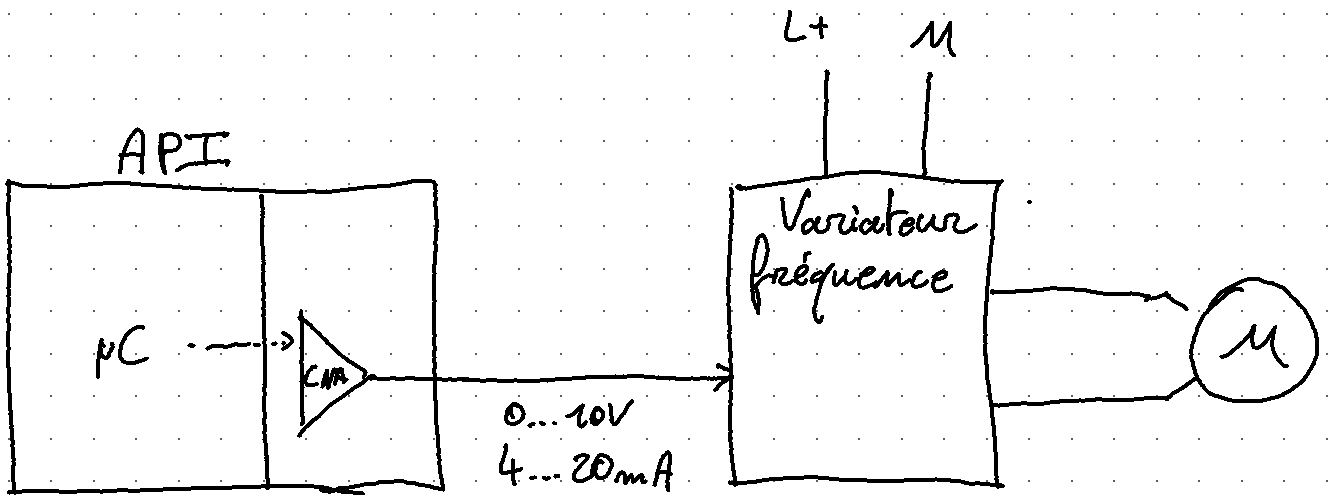
\includegraphics[height=6cm]{images/C05-CNA.png}}{\vspace{6cm}}
	\end{center}
}

\begin{UPSTIactivite}
	\UPSTIquestion{Donner la tension en sortie d'un CNA 0-10V 10 bits ayant pour valeur numérique 0b10 0000 0110}
	\vspace{2cm}
	\UPSTIquestion{Donner le courant en sortie d'un CNA 4-20mA 10 bits ayant pour valeur numérique 0b00 0001 1000}
	\vspace{2cm}
\end{UPSTIactivite}

\pagebreak
\section{Synthèse sur les entrées et sorties d'un API}

Une maquette présente à l'IUT représente le fonctionnement d'un système de stockage de pièces entre deux chaines de production (une chaine qui produit des )

\begin{UPSTIactivite}
	On désire implémenter le fonctionnement suivant :
	\begin{enumerate}
		\item A l'appui sur un bouton poussoir :
		      \begin{itemize}
			      \item Un contacteur se ferme afin d'alimenter électriquement les éléments du système
			      \item Un moteur se met en route afin de mettre en mouvement le convoyeur (tapis roulant).
		      \end{itemize}
		\item Un bouton d'arrêt d'urgence normalement fermé permet de couper l'alimentation.
	\end{enumerate}

	\UPSTIquestion{Lister les éléments nécessaires au fonctionnement de ce système}
	\vspace{2cm}
	\UPSTIquestion{Dessiner un cablâge permettant ce fonctionnement sur un Logo}
	\vspace{11cm}
\end{UPSTIactivite}

\end{document}
